\documentclass[twoside,spanish]{elsarticle}
\usepackage[T1]{fontenc}
% \usepackage[latin9]{inputenc}
\pagestyle{headings}
\usepackage{float}
\usepackage{amstext}
\usepackage{amsthm}
\usepackage{amssymb}
\usepackage{graphicx}
\PassOptionsToPackage{normalem}{ulem}
\usepackage{ulem}

\makeatletter

\floatstyle{ruled}
\newfloat{algorithm}{tbp}{loa}
\providecommand{\algorithmname}{Algoritmo}
\floatname{algorithm}{\protect\algorithmname}

\theoremstyle{plain}
\newtheorem{thm}{\protect\theoremname}
\theoremstyle{definition}
\newtheorem{defn}[thm]{\protect\definitionname}

\usepackage{algorithm}
\usepackage{algpseudocode}

\journal{Curso de <<Análisis de algoritmos>>, PUJ, Bogotá, Colombia - }


\makeatother

\usepackage[spanish]{babel}
\addto\shorthandsspanish{\spanishdeactivate{~<>}}

\providecommand{\definitionname}{Definición}
\providecommand{\theoremname}{Teorema}

\begin{document}

\begin{frontmatter}{}

\title{Algoritmo para solucionar las ``Torres de Hanoi''\tnoteref{t1}}

\tnotetext[t1]{Este documento presenta la escritura formal de un algoritmo que soluciona
el juego de las Torres de Hanoi.}

\author[lfv]{Leonardo Flórez-Valencia}

\ead{florez-l@javeriana.edu.co}

\address[lfv]{Pontificia Universidad Javeriana, Bogotá, Colombia}

\begin{abstract}
En este documento se presenta la escritura formal del problema ``calcular
la secuencia de pasos para resolver el juego de las Torres de Hanoi'',
junto con un algoritmo de solución.
\end{abstract}

\begin{keyword}
algoritmo, escritura formal, Torres de Hanoi.
\end{keyword}

\end{frontmatter}{}

\section{Análisis del problema}

Se desea escribir un algoritmo informar la secuencia de pasos que
resuelven el juego de las torres de Hanoi. Antes de proponer dicha
solución algorítmica, primero es importante describir el juego.

\begin{defn}
Las Torres de Hanoi es un rompecabezas o juego matemático inventado
en 1883 por el matemático francés Édouard Lucas. Es un juego de un
jugador que consiste en un número de discos perforados de radio creciente
que se apilan insertándose en uno de las tres torres fijadas a un
tablero. El objetivo del juego es trasladar la pila a otro de los
postes siguiendo las reglas:
\end{defn}

\begin{enumerate}
\item solo se puede mover un disco a la vez y
\item no se puede colocar un disco más grande encima de un disco más pequeño
\end{enumerate}

Un esquema de un estado del juego se presenta a continuación:
\begin{center}
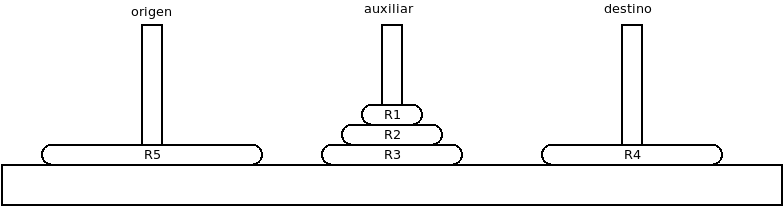
\includegraphics[width=0.75\textwidth]{hanoi_schema}
\par\end{center}

De esta descripción del juego se puede concluir:
\begin{enumerate}
\item La cantidad de discos es finita y contable, entonces es un número
natural $n\in\mathbb{N}$.
\item El radio exacto de cada disco es irrelevante, lo único relevante es
un dato que permita ordenar los discos, entonces el radio de cada
disco se puede representar con un número natural $r\in\mathbb{N}$.
\end{enumerate}

\section{Diseño del problema}

El análisis anterior nos permite diseñar el problema: definir las
entradas y salidas de un posible algoritmo de solución, que aún no
está definido.
\begin{enumerate}
\item \emph{\uline{Entradas}}:
\begin{enumerate}
\item $n\in\mathbb{N}$, la cantidad de discos.
\item $\left(o,d,a\right)$, una tripleta con los identificadores de las
torres: \textbf{\emph{\uline{o}}}rigen, \textbf{\emph{\uline{d}}}estino
y \textbf{\emph{\uline{a}}}uxiliar.
\end{enumerate}
\item \emph{\uline{Salidas}}: $S=\left\langle \left(i,j\right);i,j\in\left\{ o,d,a\right\} \right\rangle $
la secuencia de pasos para solucionar el juego.
\end{enumerate}

\section{Algoritmo de solución}

El algoritmo de solución se basa en una estrategia de solución recurrente,
donde se busca mover todos los discos superiores a la torre auxiliar,
para luego mover el disco más grande al destino.

\begin{algorithm}
\begin{algorithm}[H]

\begin{algorithmic}[1]

\Require{$n\in\mathbb{N}$, the number of disks to move}

\Require{$t\equiv\left(o,d,a\right)$, a tuple with the three towers
(\textbf{\emph{\uline{o}}}rigin, \textbf{\emph{\uline{d}}}estination
and \textbf{\emph{\uline{a}}}uxiliary)}

\Procedure{SolveTowersOfHanoi}{$n,t\equiv\left(o,d,a\right)$}

  \If{$n=1$}

    \State\Return$\left\langle t\right\rangle $

  \Else

    \State$M\leftarrow\emptyset$

    \State$M\leftarrow M\bigcup\text{\Call{SolveTowersOfHanoi}{\ensuremath{n-1,\left(o,a,d\right)}}}$

    \State$M\leftarrow M\bigcup\text{\Call{SolveTowersOfHanoi}{\ensuremath{1,\left(o,d,a\right)}}}$

    \State$M\leftarrow M\bigcup\text{\Call{SolveTowersOfHanoi}{\ensuremath{n-1,\left(a,d,o\right)}}}$

    \State\Return$M$

  \EndIf

\EndProcedure

\end{algorithmic}

\end{algorithm}

\caption{Solucionador de las Torres de Hanoi}

\end{algorithm}


\subsection{Invariante}

La secuencia de movimientos se actualiza respetando las reglas del
juego.

\subsection{Análisis de complejidad}

El algoritmo exhibe una complejidad $O\left(2^{n}\right)$.

\subsection{Notas de implementación}

La secuencia de retorno $M$ debe ser implementada con una estructura
lineal estilo ``lista de tuplas''. Los identificadores de las torres
deben ser representados por valores finitos contables (números naturales
o enteros o cadenas de caracteres).
\end{document}
